\textbf{Note: What not developed here should go into a final ``Further studies'' section or similar.}

\section{An intro chap on motivation and experiments?}
\begin{itemize}
  \item Time crystals?
  \item Time-resolved diffraction patters, temporal double slit experiment + Muga theory \url{https://arxiv.org/pdf/0812.3034.pdfß}
\end{itemize}

%\clearpage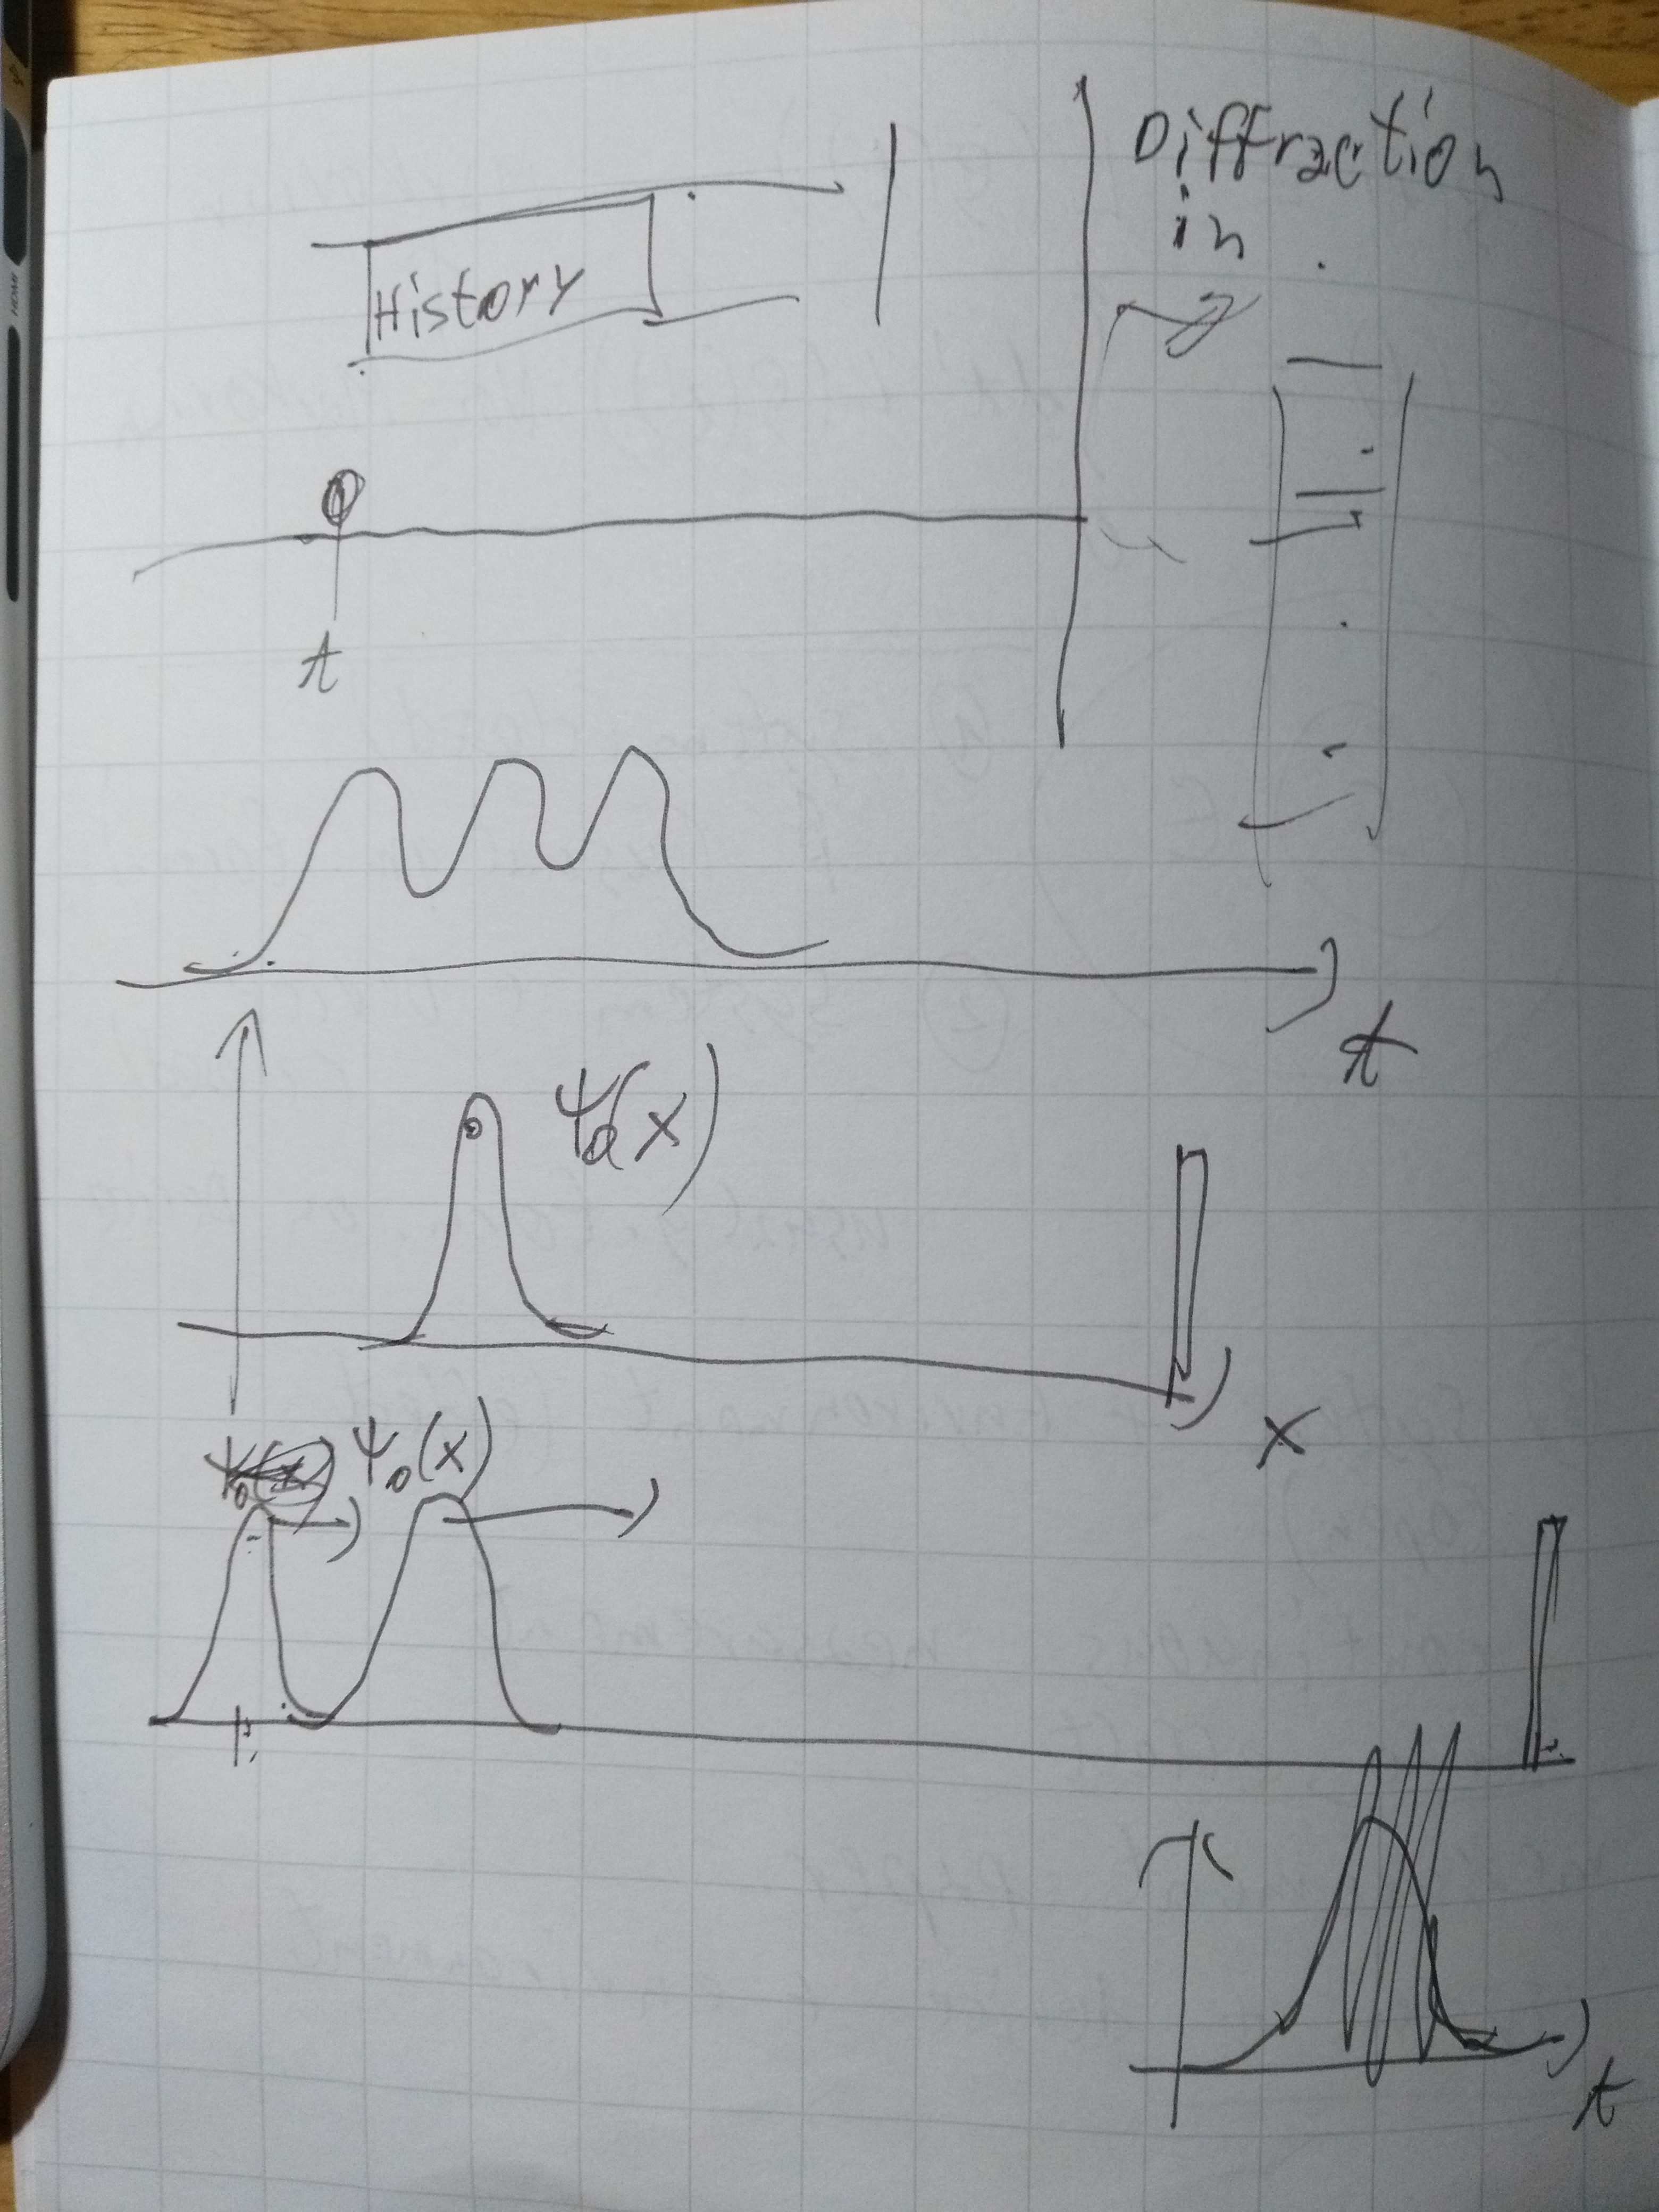
\includegraphics[width=\linewidth]{img/diffraction.jpg}

\section{Misc}

\subsection{Quantum computing, IBM, decomposition, Trotter-SUzuki, Sine-cosine, qubiter dir}

Previous section(s) read(s):
\begin{quote}
  A benefit of finite-dimensional systems is the potential implementation on a finite array of
  qubits in a quantum computer.
\end{quote}
Make a ref from there to here, and talk about qubiter and stuff.

Also, \cite{Moreva:illustration} has FIG.1 gate array repr\dots

\subsection{Quantum Blockchain and Entanglement in Time}

\url{https://spectrum.ieee.org/tech-talk/computing/networks/quantum-blockchains-could-act-like-time-machines}
\url{https://arxiv.org/abs/1804.05979}


\subsection{Misc}

Extra: \cite{TimeAnyons}.

TQM Book: time of residence: applicable to qubits, therefore Moreva experiment.

\url{https://arxiv.org/abs/1708.04302} majorization, thermo.


\subsection{and dwell time}

\cite[\S 5]{TQM2}, \cite{YearsleyHalliwell_Clocks}. (create an @inbook for this)

\subsection{In relation with the \term{time of residence}}

Here we compare \cite{Moreva:synthetic, Moreva:illustration}
(a Page and Wootters problem)
with the ``standard'' \term{time of residence}
treated in \cite[\S 5.5.2]{TQM2} (create an @inbook for the chapter), 
the only usable concept since there is no notion of position
for a qubit.

\subsection{Comparison with (Kijowski/Aharonov-Bohm) time of arrival}

Time of arrival is derived for non-relativistic \parencite{Delgado_TOA, Delgado_TOA2}
and relativisitic \parencite{Leon_TOA_R}
particle.

Kijowski: \cite{Kijowski_Time, Kijowski_Comment}.

\subsection{In relation to Leggett-Garg inequalities}
(Also mentioned in \cite{Moreva_position}).

Ref \cite{LeggettGarg+PageWootters}.

But also Lloyd: \url{https://arxiv.org/abs/1608.05672},
\emph{Decoherent histories approach to the cosmological measure problem}.
Lindbladt, Markov, Open Systems.

Halliwell, \url{https://arxiv.org/abs/1604.01659}. Ancilla, decay (spontaneous emission?).

A phylosophical object to decoherent histories / Everett (Everett mentioned in Marletto/ref)
is at
\url{https://arxiv.org/abs/1603.04845}.



\subsection{On ``taking time seriously'' (time is real) and why it can still be real in Page and Wootters}

No, Smolin
(\term{Time Reborn}, \term{The Singular Universe and the Reality of Time})
pushes this too far, even Special Relativity's time is too ``virtual'' for him.
Similarly, the philosopher Tim Maudlin

\url{https://www.quantamagazine.org/a-defense-of-the-reality-of-time-20170516/}

Here instead we just argue that the clock can actually be really time, not any observable.
We use notation $T$ as in time instead of $C$ as in clock etc.

In this sense, the Moreva experiment is a quantum analogue simulation.


\section{Time crystals}

References: \cite{crystal2,crystal3,crystal2012}.


\section{Irrev}

\cite[\S IV.  UNBOUNDED-ENERGY CLOCKS?]{Maccone:Pauli}

\subsection{Use open quantum systems theory in ``Decoherence and measurement'' chapter + Entropy}
Schmidt decompositions, spatial and temporal states in
$\hilb{H}_T$ and $\hilb{H}_S$
are described as density operators
(mixed states).

This has been actually used to prove clock time-frequency uncertainty relation
in terms of mixture.

What if there isn't a ``perfect entanglment'' between space and time.

Use the Von Neumann entropy (or other methods) to quantify entanglement?

When the entanglement is perfect, the notion of time evolution emerges, just
like between two dimensions in space, it may or may not ``emerge'' that
$y$ ``depends'' upon $y$ for a given distribution of positions.

Where the entanglment is maximal, the Von Neumann entropy is also maximal.

Arrow of time as increasing entanglement (and entropy!). See Also
\cite{Marletto:Evolution}.

Also Lloyd recent on entropic uncertainty (for time\dots \cite{Lloyd:Entropic}).
Maybe also \cite{Wehner:Uncertainty}.

Subadditivity.

\section{Entanglement and decoherence (Arrow of time)}
See also \cite{EntanglementVsDecoherence}.

Decoherence is an irreversible process, it also happens in measurement.

According to Marletto and Vedral, arrow of time is increase in Entanglement
between the clock and the rest.

So, there seems to be a contradiction: is entanglement ``decreasing''
(i.e. destroyed by decoherence) with time
or increasing?

We can avoid the contradiction saying that
entanglement between two finite systems is
destroyed while the entanglement of each of them with the universe
is increasing.

\subsection{``Harmonic clocks''}

Use the harmonic oscillator in \cite{HarmonicClocks}
as a PaW clock for the same packet that is measured in
Ruschhaupt's detector model.

Therein, fading wave function: is minus derivative an event?
L4 normalized?


\subsection{Misc}

Idea: use section B ``Measurement'' of \cite{Lloyd:Time}: detector as (binary) measument device.

``Philospher'': \url{https://arxiv.org/abs/1704.07236}.

Time of arrival and clocks: again, \cite{YearsleyHalliwell_Clocks}.
Which maybe suggests we should not worry too much of $H\ket{\Psi} = 0$.

We don't.

BUT please note \cite{YearsleyHalliwell_Clocks} uses a clock that is
\emph{coupled} with the system, while in PaW they are ``only'' entangled.
So their calculation may be unnecessarily complicated.
Maybe the weakjly coupling case can be used?

Other systems of interest: decays. Prvanovic new.

Reference \cite{ConnesRovelliThermo}.

Relate with John Goold's works? The ancilla as a clock? --- Topical Review

Markovianity, histories.

Lloyd on arXiv: from clock to cloners; erasing; scrambling (as in Goold).

Lloyd on decoherent histories (Gellman, Hartle?).

Dechoerence / irreversibility / measurement.

Vedral / Lloyd. Discord.

Measuring entanglement: Quantification of Concurrence via Weak Measurement: 1611.00149.

Marletto/Vedral on Arrow of time. Arrow of time as increasing entanglement.

Arrow of time:

\url{https://www.wired.com/2014/04/quantum-theory-flow-time/}

\url{https://en.wikipedia.org/wiki/Loschmidt%27s_paradox}

\url{https://www.quantamagazine.org/20160119-time-entanglement/}

\url{https://arxiv.org/pdf/1702.07706.pdf} \textit{The second law of thermodynamics at the microscopic scale}
Thibaut Josset,
Aix Marseille Univ. (David).

Maxwell's demon: https://arxiv.org/pdf/1702.05161.pdf

\subsection{and paths}

Both \cite{YearsleyHalliwell_Clocks} and \cite{Gambini_PW}
reason in terms of paths and actions, maybe Feynmann stuff
in following chapter... and maybe conistent historiesapproach can help
towards linking PaW and ToA?

Also \url{http://quantum.phys.cmu.edu/CHS/CHS_transp.pdf}.

\subsection{Decays?}

We might want to look at exponential decay from \url{https://arxiv.org/abs/1704.07236},
then compare with exponential decay with P and W using Lloyd Giovannetti and Maccone (ref).

\subsubsection{Purification}

See https://arxiv.org/pdf/quant-ph/0512125.pdf, P-W time as a purifying ancilla
of the (Kijowski?) time.

\section{Misc/Multi/Extras/Outlook}

\url{https://arxiv.org/abs/1703.05876}
--- \emph{comment}: time measured and stored here
may be all classical information
so this paper may or may not be relevant for the topic.

But
``prototypes of clocks based on quantum principles,
such as entanglement and squeezing''
may make this interesting again, see reference therein.
They also cite Lloyd, Giovannetti and Maccone,
but a paper quite older than \cite{Lloyd:Time}.

\url{https://arxiv.org/abs/1603.02522}
\emph{Decoherence by spontaneous emission: a single-atom analog of superradiance}.
Decoherent histories, non-markovianity, open quantum systems.

\url{https://arxiv.org/abs/1007.2615} Time travel / Quantum CTC.

Carmichael et al. \cite{CarmichaelOQS2017} (Andreas's reading)
(non-markovianity).

Non-markovian, quantum-to-classical, open systems, David,
\url{https://arxiv.org/pdf/1703.09428.pdf}.

In his works, Zurek mentions:
DeWitt, Everett, gell_Mann, hartl, Many Worlds, consistent/decoherent histories:
idea: Lagrangian over a history? Principle of least action?

Zurek: ``Reduction of the Wavepacket: How Long Does it Take?'' (arxiv),
``quantum''' time? \cite{Zurek_Einselect} also mentions
``decoherence timescale''.

Von Neumann/Shannon entropy in measurement? Mention information problems
in quantum cosmology (where a quantum time is necessary)? Etc. etc.

\section{for Relativistic treatment}

Lorentz (+Galilei?) transformation. Lorent/Poincare groups. May be Important:
see \cite{LocalizationEntanglmentRelativistic}.

\cite{RealisticClocks}.

\cite{HarmonicClocks} concludes ``Classical clock can be described by an Hamiltonian linear in momentum''\dots
like in relativity?

\cite{Lloyd:Time} does not only deal with improper eigenstates in $\hilb{H}_T$
(full evolutions?)
but also normalized ones (in $\hilb{H}_T$! \emph{``Events''}?)

A Page and Wootters time of arrival is mentioned in \cite{Gambini_PW}.

\subsection{Time-of-arrival for a Klein-Gordon free particle}

See \cite{Galapon_KG}.

\subsection{Feynmann path stuff}

Sokolovski 1703.01966, Feynmann paths...\subsection{(dis)entanglement under gravity, decoherence, event formalism}

1703.08036 An experiment to test decoherence under gravity aka entangled photons undergoing different paths and how their entanglement is affected.
``Space QUEST mission proposal: Experimentally testing decoherence due to gravity''.

Are they getting entangled with the environment instead? (Merletto and Vedral).

The theoretical paper behind the space experiment: \url{https://arxiv.org/pdf/1406.3677.pdf}. Interestingly, it mentions 
\emph{event formalism}, and we thought about that: is an event something
representable as a proper vector in $\mathcal{L}^2(\mathbb{R}^4)$ --- where one of the dimensions is time?
Deepen the event formalism if it's quantum.

Resume ``Quantum Statistical Gravity''? \url{https://arxiv.org/abs/1602.05707}.

``Fundamental decoherence from quantum gravity: a pedagogical review''
\url{https://arxiv.org/abs/gr-qc/0603090} ---
``fundamental loss of unitarity
that appears in quantum mechanics
due to the use of a physical apparatus to measure time''.

Closed timelike curves are also the subject of a paper by Lloyd (cite!).

``Deutsch argued that
the usual paradoxes associated with such solutions of general
relativity can be resolved by quantum mechanics''  in the reference above. But in the even formalism
\emph{spacetime is still a classical background!}. Event operators a parametrized by $t$\dots

\subsection{Prvanovic and P\&W}
In \cite{Prvanovic}, essentially the clock observable is the Hamiltonian.
The two example clocks are an harmonic oscillator and a free particle.
The harmonic oscillator features discrete time. Generally a time which is
{bounded from below}
is consistent with the Big Bang...

Prvanovic uses ``relativisitc'' constants...

BTW, please note a time bounded from below WOULD NOT be sufficient to overcome the Pauli objection alone.

\section{Photon position}

Quantum mechanics is a 0+1 QFT \parencite{QFT_0+1}.
The \emph{dimension} of the field theory is the number of external parameters.
The P-W mechanism ``quantizes'' external parameters, or make their property
of classical external parameter \emph{emerge} out of a quantum observable
of an entangled subsystem (where there exists a Schmidt decomposition over
eigenstates of said observable).

In this sense, time in quantum mechanics is like time \emph{and position}
in quantum field theories such as quantum optics or the Standard Model.

We can imagine P-W ``meter sticks'' instead of clocks, to measure
photon position and thus tackle the same problem of \cite{HawtonPhotonPosition}.

\section{Photon \emph{absorption}}

Photons are physically/really absorbed (or \emph{emitted}), although under a different theoretical framework
(second quantized Vs QM). No need of complex potentials\dots Connect with spontaneous emission?

Spontaneous emission/decay compared with PW (Maccone) and Kiukas (detection).
Perhaps Prvanovic article on spontaneous decay?
